\chapter{Methodology}

In this chapter we will go over the methods used to build and train our own pose estimation model.

\section{Fully Rendered Datasets: ScrewDataset}

We find ourselves in the situation where we want to train a 6D pose estimation model on a certain set of objects, that are not present in any available dataset. This necessarily means that we must create our own datasets for training and evaluation.

To create these we require images with their associated ground truths. However, collecting this data in the real world is tedious and difficult, considering that any errors or biases will affect the perfomance of the final model. 

One possible solution is to use rendering software, which can generate potentially infinite quantites of training images. However, while a model trained on this data could certainly work well in simulation, we have no guarantee whether it would also function in real life. This is because a simulated sensor and simulated enviroment are unable to reproduce unmodeled physical effects and noise in the same way an optical sensor would. This issue is dubbed the "reality gap"\cite{domainRandomization2}, and there are various ways we could attempt to solve it.

Domain Randomization\cite{domainRandomization} is the most readily available method for bridging this gap. The hypothesis behind this concept states that introducing sufficient variability in the simulated domain will allow the model to generalise to the real world with no additional training. In our situation, the domain is an image, so we have huge liberty in choosing how to randomize it.

\subsection{Generation Methodology}

For our first attempt, we decided to generate a dataset for estimating the pose of a single object: a standard M6x30 hexagonal head screw. This is a very challenging object for pose estimation, as it is small (34 mm in length) and symmetric. The reason why symmetric objects are difficult for pose estimation is explained in depth in appendix A.2.

To render the images in our dataset, we use Unity's Perception package\cite{unityPerception}, which integrates domain randomization features into its pipeline. Unity Perception works by simulating a scene, and then rendering each simulated frame from the perspective of a camera. Within each scene there are various objects, including the 3D model of the dataset items, and the camera itself. 

One particular object connected to the scene is the scenario, which is in turn connected to a set of scripts called randomizers. When we simulate a scene, the scenario specifies the number of iterations and the number of frames we want to render for each iteration. At the beginning of each iteration, all randomizers connected to the scenario are called to set one of the domain variables, which can be anything within the scene, from positions and rotations of objects to their textures and colors. The camera then renders the scene from its perspective, and saves both the image and its associated annotations.

\begin{figure}
    \centering
    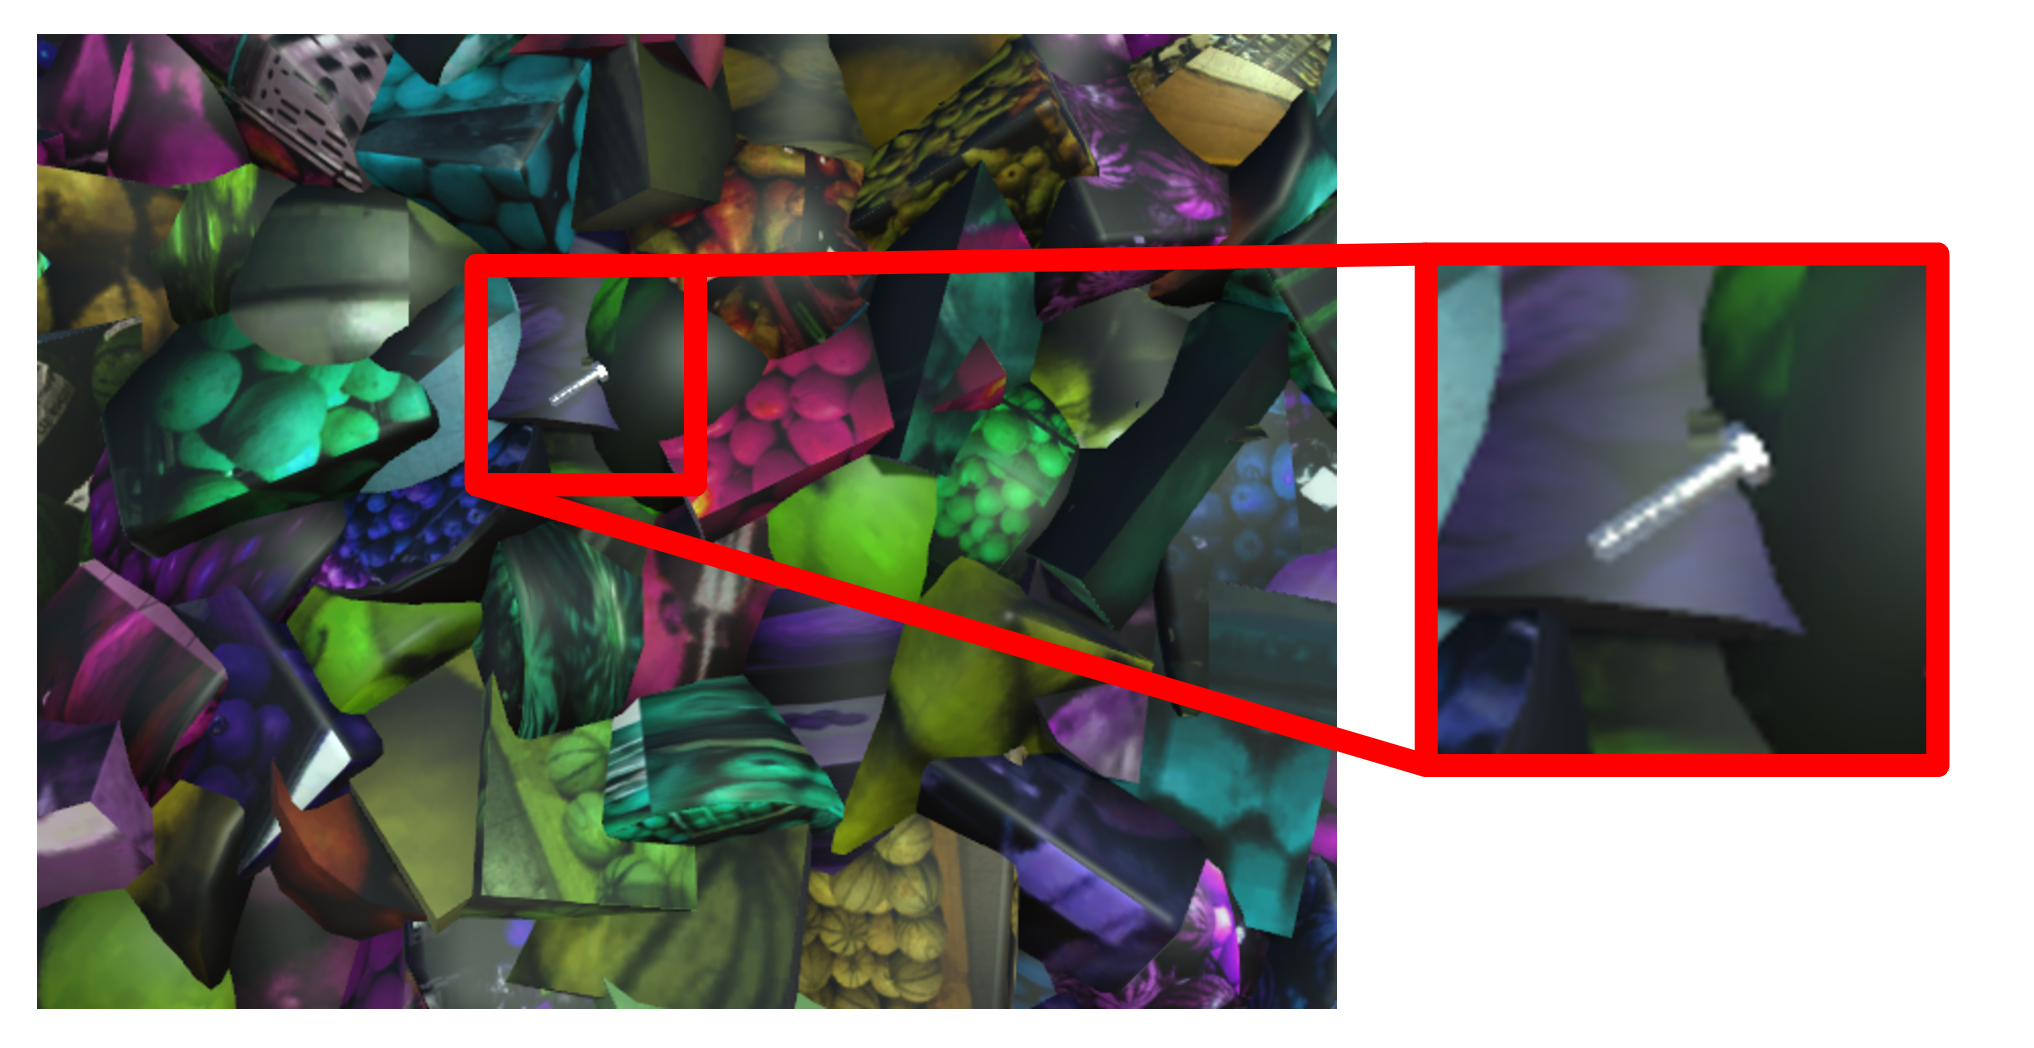
\includegraphics[width=0.6\textwidth]{screwdataset/ScrewDataset.png}
    \caption{One of the images generated with Unity's Perception package for training our model, with a zoom-in on the screw.}
    \label{fig:screwdataset}
\end{figure}

For our dataset, we implemented a scenario with 10'000 iterations lasting one frame each. We used a model of the M6x30 screw obtained from the FreeCAD Fasteners workbench\cite{Fasteners}, and then used a custom randomizer to set its position and rotation for each iteration. We then used default randomizers provided as samples by Unity as part of its Perception package to generate a background, composed by random 3D shapes placed with random positions, orientations and textures. Finally, we used a custom randomizer to set the lighting color, intensity and origin. A sample image from this dataset appears in figure \ref{fig:screwdataset}.

We then converted the Unity output to a format that we could feed to EfficientPose for training. This required converting the ground truths from Unity's internal left-handed reference system to the right-handed reference used by the rest of the world, and generating other relevant information required by EfficientPose, such as mask information and the dimensions, center and diameter of the 3D bounding box enveloping the model of the screw. To do this, we automated the procedure taking LINEMOD as a reference.

In this manner we can quickly and easily generate arbitrarily large datasets for training, by first running the scenario inside unity, and then running the conversion script for EfficientPose. Since the final dataset contains 10'000 images of a screw, in a fit of originality we decided to name it "ScrewDataset" and we will be referring to it as such in the rest of this thesis.

\subsection{Training}

The original version of EfficientPose is trained on LINEMOD. However, the dimensions of LINEMOD and of our own dataset are completely different: LINEMOD has around 1200 images per object, and only about 200 of these are used for training, while ScrewDataset has exactly 10000 images, 9000 of which are used for training. This means that we have to tweak the training parameters to our own dataset. In this subsection we will go over these tweaks and what they signify.

First, we reduced the number of epochs from 5000 to 100. Since our dataset contains 45 times more images, these two values represent a similar training time for the two different datasets. EfficientPose also by default evaluates the model only every 10 epochs due to the small epoch size; we change this value to evaluate at the end of every epoch.

Due again to the small amount of samples, EfficientPose includes a couple of intelligent data augmentation techniques: one to randomly rescale and rotate the input image (6DoF augmentation), and another to change its colors and grain\cite{RandAugment}. However, we will not be implementing these methods with ScrewDataset, due to both the amount of input images and the fact that we already randomize position and colors in generation.

EfficientPose implements Keras' ReduceLRonPlateau callback. This is standard practice: large learning rates quickly adjust the model but can lead to fluctuations, local minima and divergence; smaller learning rates mean the model takes an excessive amount of time to improve\cite{ReduceLR}. Thus this callback automatically reduces the learning rate when the model stagnates, thus maintaining a value closer to ideal during training. By default, EfficientPose halves the LR every time the accuracy does not improve for 25 epochs; we changed this to 20 percent every 5 epochs to account for the increased number of samples per epoch.

Finally, a quality of life change. EfficientPose is concieved to be trained in a single sitting: interrupting and restarting training does not maintain the learning rate, optimizer state and momentum, leading to a rise in training loss before it starts diminishing again after a few epochs. Since we do not want to train the model consecutively for days on end, we implemented custom callbacks that save the optimizer state and learning rate, thus we haveintroducing the possibility of interrupting and resuming training if necessary.

\subsection{Results}

\section{Partially Rendered Datasets: ScrewPose}

\section{Refinement with ICP}